\vspace{10pt}

{\centering\subsection*{何宇州:读《钢铁是怎样炼成的》有感}}

\addcontentsline{toc}{subsection}{何宇州:读《钢铁是怎样炼成的》有感}

\renewcommand{\leftmark}{何宇州:读《钢铁是怎样炼成的》有感}

\begin{figure}[htbp]

\centering

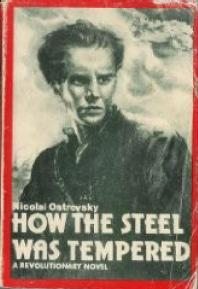
\includegraphics[width = .5\textwidth]{./ch/42.jpg}

\end{figure}

《钢铁是怎样炼成的》这本小说的作者是奥斯 特洛夫斯基,保尔·柯察金是这本书的男主角,小说中的事件都是他的亲身经历。经历了工作、家庭、爱情、朋友的种种考验,保尔他从一个普通的老百姓变成了一个十分优秀的红军战士。之后因为战争全身瘫痪,导致他双目失明,无法与正常人一样。但是他都一直保持着乐观、开朗, 为了革命奋不顾身。看了这本小说,我觉得保尔能承受这么多的痛苦太了不起了。    

这本书写了保尔的一生, 写了他如何从一个非常普通的人变成了一位与命运对抗的战士。他为了和平,多次重伤,最后他因为不能下战场,不能工作多次想自杀,但是他还是想通了。他让别人帮他写小说,他的第一本小说出版之后,他就开始大量的写小说。 

文中最令我印象深刻的那一篇文章,就是钢铁意志。保尔在园中散步的时候,他感到脊椎一阵剧痛,之后就摔倒在地上,他费了好大劲才回到屋子里。第二天,医生给他做了详细的检查,发现他脊椎有一个深坑,可保尔非常平静。医生惊讶的问说:“你背上有一个深坑,以前有没有发作过。”保尔淡定的回答说:“从来都没有。”医生又说:“希望它以后再也不会发作,脊椎可不喜欢。”这一段中医生检测到保尔身上有很多重伤。保尔却没有说过痛。我看完这一段后对保尔产生出了深深的敬畏。

《钢铁是怎样炼成的》这本小说不仅是上辈人们所喜爱的著作,它还是我们现代少年的照明灯。保尔的光辉形象一直活在我们心里。


\vspace{10pt}

作者:五(3)班何宇州

指导老师:刘婷



投稿:2021年4月13日

发表:2021年4月15日











                



\vspace{10pt}

\hline

